\chapter{\IfLanguageName{dutch}{Stand van zaken}{State of the art}}%
\label{ch:stand-van-zaken}

% Tip: Begin elk hoofdstuk met een paragraaf inleiding die beschrijft hoe
% dit hoofdstuk past binnen het geheel van de bachelorproef. Geef in het
% bijzonder aan wat de link is met het vorige en volgende hoofdstuk.

% Pas na deze inleidende paragraaf komt de eerste sectiehoofding.

% Dit hoofdstuk bevat je literatuurstudie. De inhoud gaat verder op de inleiding, maar zal het onderwerp van de bachelorproef *diepgaand* uitspitten. De bedoeling is dat de lezer na lezing van dit hoofdstuk helemaal op de hoogte is van de huidige stand van zaken (state-of-the-art) in het onderzoeksdomein. Iemand die niet vertrouwd is met het onderwerp, weet nu voldoende om de rest van het verhaal te kunnen volgen, zonder dat die er nog andere informatie moet over opzoeken \autocite{Pollefliet2011}.

% Je verwijst bij elke bewering die je doet, vakterm die je introduceert, enz.\ naar je bronnen. In \LaTeX{} kan dat met het commando \texttt{$\backslash${textcite\{\}}} of \texttt{$\backslash${autocite\{\}}}. Als argument van het commando geef je de ``sleutel'' van een ``record'' in een bibliografische databank in het Bib\LaTeX{}-formaat (een tekstbestand). Als je expliciet naar de auteur verwijst in de zin (narratieve referentie), gebruik je \texttt{$\backslash${}textcite\{\}}. Soms is de auteursnaam niet expliciet een onderdeel van de zin, dan gebruik je \texttt{$\backslash${}autocite\{\}} (referentie tussen haakjes). Dit gebruik je bv.~bij een citaat, of om in het bijschrift van een overgenomen afbeelding, broncode, tabel, enz. te verwijzen naar de bron. In de volgende paragraaf een voorbeeld van elk.

% \textcite{Knuth1998} schreef een van de standaardwerken over sorteer- en zoekalgoritmen. Experten zijn het erover eens dat cloud computing een interessante opportuniteit vormen, zowel voor gebruikers als voor dienstverleners op vlak van informatietechnologie~\autocite{Creeger2009}.

% Let er ook op: het \texttt{cite}-commando voor de punt, dus binnen de zin. Je verwijst meteen naar een bron in de eerste zin die erop gebaseerd is, dus niet pas op het einde van een paragraaf.

\section{Computatie op het web}

Computatie op het web werd voorheen in beperkte mate uitgevoerd met WebGL deze is gebaseerd op de OpenGL standaard. WebGL 2.0 laat toe om berekeningen uit te voeren en hierbij de parallelle rekenkracht van grafische processors te gebruiken. Wanner de grafische rekenkracht van een GPU wordt ingezet om algemene calculaties uit te voeren is er sprake van \textit{general purpose graphics processing unit} ook wel \textit{GPGPU} genoemd.

\begin{displayquote}
    "The basic realization to understanding GPGPU in WebGL is that a texture is not an image, it's a 2D array of values." \autocite{Tavares2021}
\end{displayquote}

WebGL gebruiken voor GPGPU is echter een complexe implementatie die gebruik maakt van een \textit{global state} die volgens \textcite{Surma2022} al snel kan leiden tot complexe code en hierdoor dus ook tot fouten. De implementaties van GPGPU wed door de introductie van \textit{Transform Feedback} in WebGL 2.0 toegankelijker, maar deze nieuwere versie van WebGL werd pas recent ondersteund door \textit{Apple} op \textit{Safari} in september 2021.

\begin{figure}
    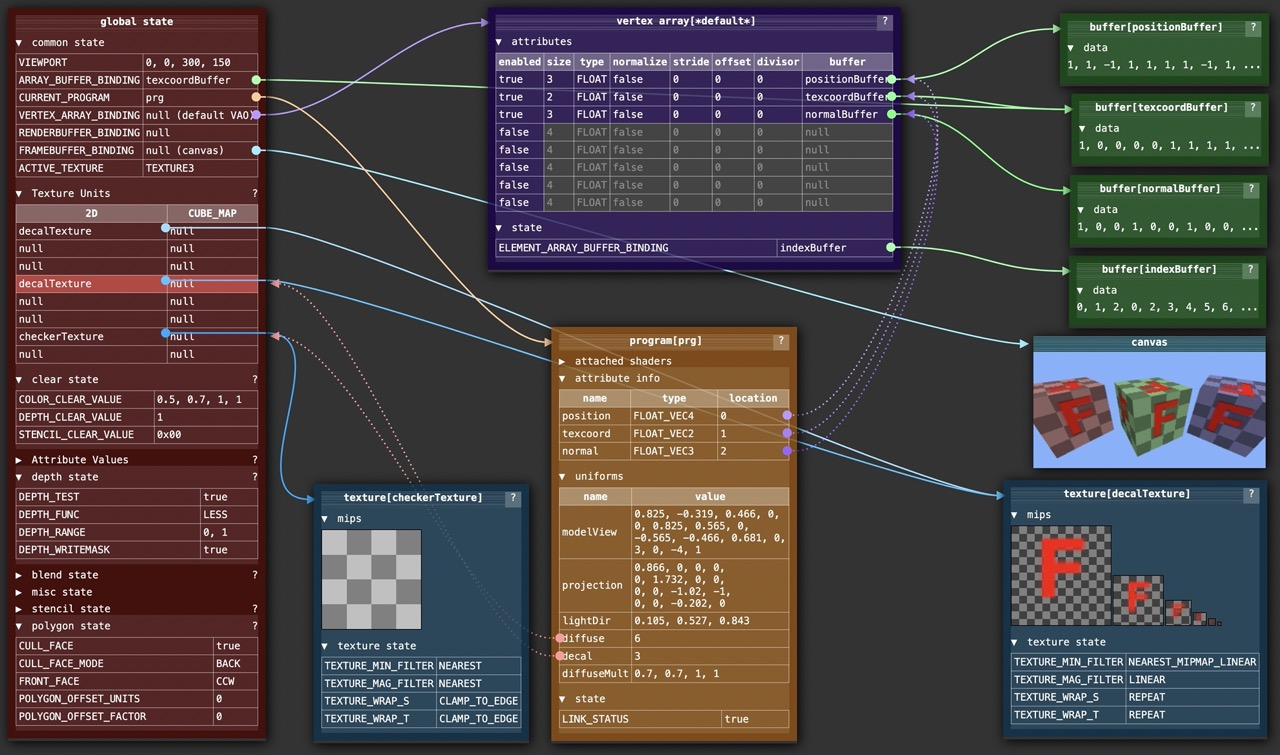
\includegraphics[width=\linewidth * 3 / 4]{WebGLAndGlobalState.jpeg}
    \caption{De \textit{Global State} in \textit{WebGL}}{De \textit{Global State} in \textit{WebGL}}
    \label{fig:WebGL Global State}
\end{figure}

\bigbreak{}

Afbeelding \ref{fig:WebGL Global State} toont de \textit{global state} die gebruikt wordt in WebGL.

\bigbreak{}

Het gebruiken van WebGL voor GPGPU is niet enkel complex, het is ook een inefficiënt. Data moet eerst als een \textit{texture} worden gecodeerd daarna gedecodeerd in een \textit{shader}. Op dat moment moeten de calculaties worden uitgevoerd, deze calculaties moeten opnieuw worden gecodeerd tot een \textit{texture} alvorens met de resultaten kan worden verder gewerkt. \autocite{Surma2022}

\bigbreak{}

Deze lange onnodige complexiteit komt verder uit het feit dat WebGL werd ontworpen voor het visualiseren van grafische elementen, en dus niet om algemene computationele taken uit te voeren zoals \textit{machine learning} of het mijnen van \textit{crypto currency}. Zoals eerder vermeld verbeterde de situatie wel met WebGL 2, maar de ondersteuning voor deze API was beperkt en hierdoor kwam de proliferatie van computatie de browser niet tot stand.

\section{Introductie van WebGPU}

Omdat WebGPU wordt gestandaardiseerd door het \textit{World Wide Web Consortium}, krijgt het ook de nodige ondersteuning om een potentiele standaard te worden zoals WebGL. Een globaal innitiatief kan er dus wel toe leiden dat deze technologie een revolutie betekent voor rendering en computatie op het Web. Ook in tegenstelling tot de beperkte ondersteuning waar WebGL 2.0 op kon rekenen, zitten bij WebGPU wel alle browser fabrikanten mee in het ontwikkelingsproces. \autocite{Surma2022}

\bigbreak{}

De werking van een GPU is heel complex, hier wordt dus vaak te snel over gegaan. Er wordt door meerdere applicaties simultaan data naar het beeldscherm geprojecteerd en hierbij wordt dus de grafische kaart opgedeeld, de veiligheidsimplicaties hiervan zijn niet te onderschatten omdat deze applicaties elkaar niet mogen kunnen beïnvloeden of data van elkaar mogen uitlezen. Voor elke applicatie lijkt het dus dat deze een monopolie beschikt over de grafische kaart. Uiteraard is dit niet het geval en wordt eigenlijk de rekenkracht verdeeld. Dit leidt ertoe dat de status van uitgevoerde taken moeten worden bijgehouden omdat er altijd parallel wordt gewerkt. Programmeren voor \textit{General Purpose GPU} verloopt dus altijd op een multi threaded asynchrone manier waar dus rekening mee moet gehouden worden. \autocite{Surma2022}

\bigbreak{}

Uiteraard zijn er al meerdere implementaties van ML op de web maar deze worden beschikbaar gesteld door servers en er wordt dus nog geen gebruik gemaakt van client-sided WebGPU rendering. \textcite{Fleetwood2023a} beweert dat het essentieel zal zijn dat modellen lokaal worden gedraaid om de echte \textit{real-time} te ondersteunen.

\bigbreak{}

Ook worden er bij technologieën zoals \textit{language chain} waarbij meerdere AI-modellen serieel worden gebruikt om de functionaliteit van webapplicaties uit te breiden. Deze geweldige functionaliteit komt helaas met een grote kost aan rekencapaciteit.

\bigbreak{}

Zo merkt \textcite{Huyen2023} op in haar onderzoek dat de kost van het draaien van AI-modellen in een productie omgeving enorm hoog kan oplopen. Hierdoor komt de rendabiliteit in gevaar. Dit is echter enkel het geval wanneer modellen suboptimaal worden ingezet zoals \textcite{Fleetwood2023a} ook opmerkt.

\begin{displayquote}
    "Offloading some parts of the call chain to finetuned local models could dramatically reduce costs while offering additional benefits such as privacy and personalization." \autocite{Fleetwood2023a}
\end{displayquote}

\bigbreak{}

WGSL is helaas al opgemerkt als een moeilijke shader language om mee te werken \textcite{Madrigal2023}. Volgens Fleetwood is dit echter niet het geval en hij vindt dat de syntax toegangkelijk is omdat het veel invloeden heeft van Rust. Een populaire opkomend taaltje.

\bigbreak{}

Fleedwood beweert zelf competitie te kunnen bieden aan open AI met zijn implementatie van het FLAN-T5 model van Google. Dit uiteraard wel voor beperkte use cases maar het is toch al een goed begin.

\bigbreak{}

WebGPU laat misschien wel toe dat er rekenkracht beschikbaar wordt gesteld aan de browser maar dit wil niet zeggen dat hierdoor het probleem van draaien van lokale complexe modellen is opgelost. Er is namelijk ook een geheugen limitatie, een model moet worden ingeladen en dit liefts in VRAM van de grafische kaart. Hier kan dus potentieel een \textit{bottleneck} ontstaan. Het efficient inladen en beschikbaar stellen van deze modellen is dus essentieel. Dit stelt Fleedwood ook vast waar hij opmerkt ... 

\section{From WebGL to WebGPU}

**Global State**
Een groot probleem dat werd opgelost bij WebGPU is het verwijderen van de *global state* die beschikbaar was in WebGL, deze global state zorgde ervoor dat ontwikkelaars makkelijk fouten konden introduceren in hun code. WebGPU vervangt het global state gedrag van WebGL met pipelines die niet mutable zijn eenmaal ze zijn aangemaakt.
Deze global state zorgde erdus voor dat het maken van grote robuste applicaties moeilijk was en leide tot fragile code volgens Baufort.

-- not finished here


\section{WebGPU computations performance in comparison to WebGL} % Radin2021

Uit de ondervindingen van \textcite{Radin2021} blijkt dat WebGPU 3.5 keer sneller is dan WebGL simpele matric multiplicaties. Dit komt enerzijds omdat het proces om de berekeningen uit te voeren met WebGPU een stuk simpeler omdat WebGPU compute shaders ondersteunt en WebGL dit niet doet. Om computatie uit te voeren met WebGL is het namelijk vereist dat de data eerst wordt omgezet naar pixels zodat deze met een pixel shader kunnen worden berekent. Het nadeel hiervan is dat er een afhankelijkheid is op de canvas, omdat het gaat over het renderen van pixels. \textcite{Radin2021} ondervond hier dat WebGL de matrix multiplicatie niet ondersteund boven de 4096 bij 4096, dit komt door de fysieke limitatie van het canvas object. Maar volgens mdn web docs staat deze op 10.000 bij 10.000 tenzij de browser dit zelf limiteerd.


\section{A case for client-side machine learning} % Fleetwood2022

\textcite{Fleetwood2022} merkt op dat er een paradigm verandering aankomt in hoe ai-modellen worden getrained. De huidige techonologie werkt als volgt; een hoeveelheid informatie wordt door de gebruiker voorzien en opgestuurd naar een model dat draait in de cloud, dit model produceert een antwoord dat terug aan de gebruiker wordt voorgelegd.

\bigbreak{}

Deze paradigm is enigsinds satisch in dat het model dat draait in de cloud niet veranderlijk is. \textcite{Fleetwood2022} geloofd er in dat een toekomsige standaard met modellen die dynamish opgebouwd worden de toekoms is. Dit wil zeggen dat gewichten die worden toegepast op een AI-model gepersonaliseerd zijn voor de gebruiker.

\bigbreak{}

Het is belangrijk om hierbij de privacy aspecten te herkennen, ook valt op te merken dat computatie op het web en dus WebGPU; een kaalisator zou kunnen zijn voor zo een paradigm verandering.

\begin{displayquote}
    "It would be optimal if the subset of weights that get updated to learn about the user remained on their device." \autocite{Fleetwood2022}
\end{displayquote}

Wat \textcite{Fleetwood2022} ook opmerkt is dat er bij het draaien van een AI-technologieen vaak meerdere modellan serieel aan te pas komen. Deze modellen werken dan voort op informatie die reeds werd gegenereerd door een ander model. Deze technologie zou dus toestaan een hybride cloud te maken waarbij een deel van de computationele vereisten worden overgedragen aan de eind-gebruiker.

\bigbreak{}

Er moet wel worden benadrukt dat het downloaden van modellen een groot struikelblok voor de technologie kan betekenen. Veel modellen worden niet publiek gemaakt dus die kunnen van deze implementatie geen gebruik maken. Modellen die te groot zijn en er dus voor zorgen dat de eind-gebruiker initieel moet wachten tot deze gedownload zijn alvorens de webapplicatie volledig beschikbaar is leiden tot een gedegradeerde bruikbaarheid. Maar volgens \textcite{Fleetwood2022} zijn dit problemen die door middel van compressie en cashing grotendeels verholpen kunnen worden.

\section{WebGPU browser ondersteuning}

WebGPU wordt nog niet door alle browser ondersteund, het is dus belangrijk dat de \textit{early-adapter} gebruikers verifiëren dat hun browser compatibel is.

Dit kan makkelijk worden uitgezocht door gebruik te maken van \href{https://caniuse.com/webgpu}{caniuse.com}.

Merkwaardig is ook dat Chrome als grootste speler binnen de markt al reeds volledige ondersteuning heeft uitgevoerd in versie 113. \autocite{Deveria2024}

\bigbreak{}

Afbeelding \ref{fig:Browser Support} toont de ondersteuning voor WebGPU binnen verschillende \textit{browsers}.

\begin{figure}
    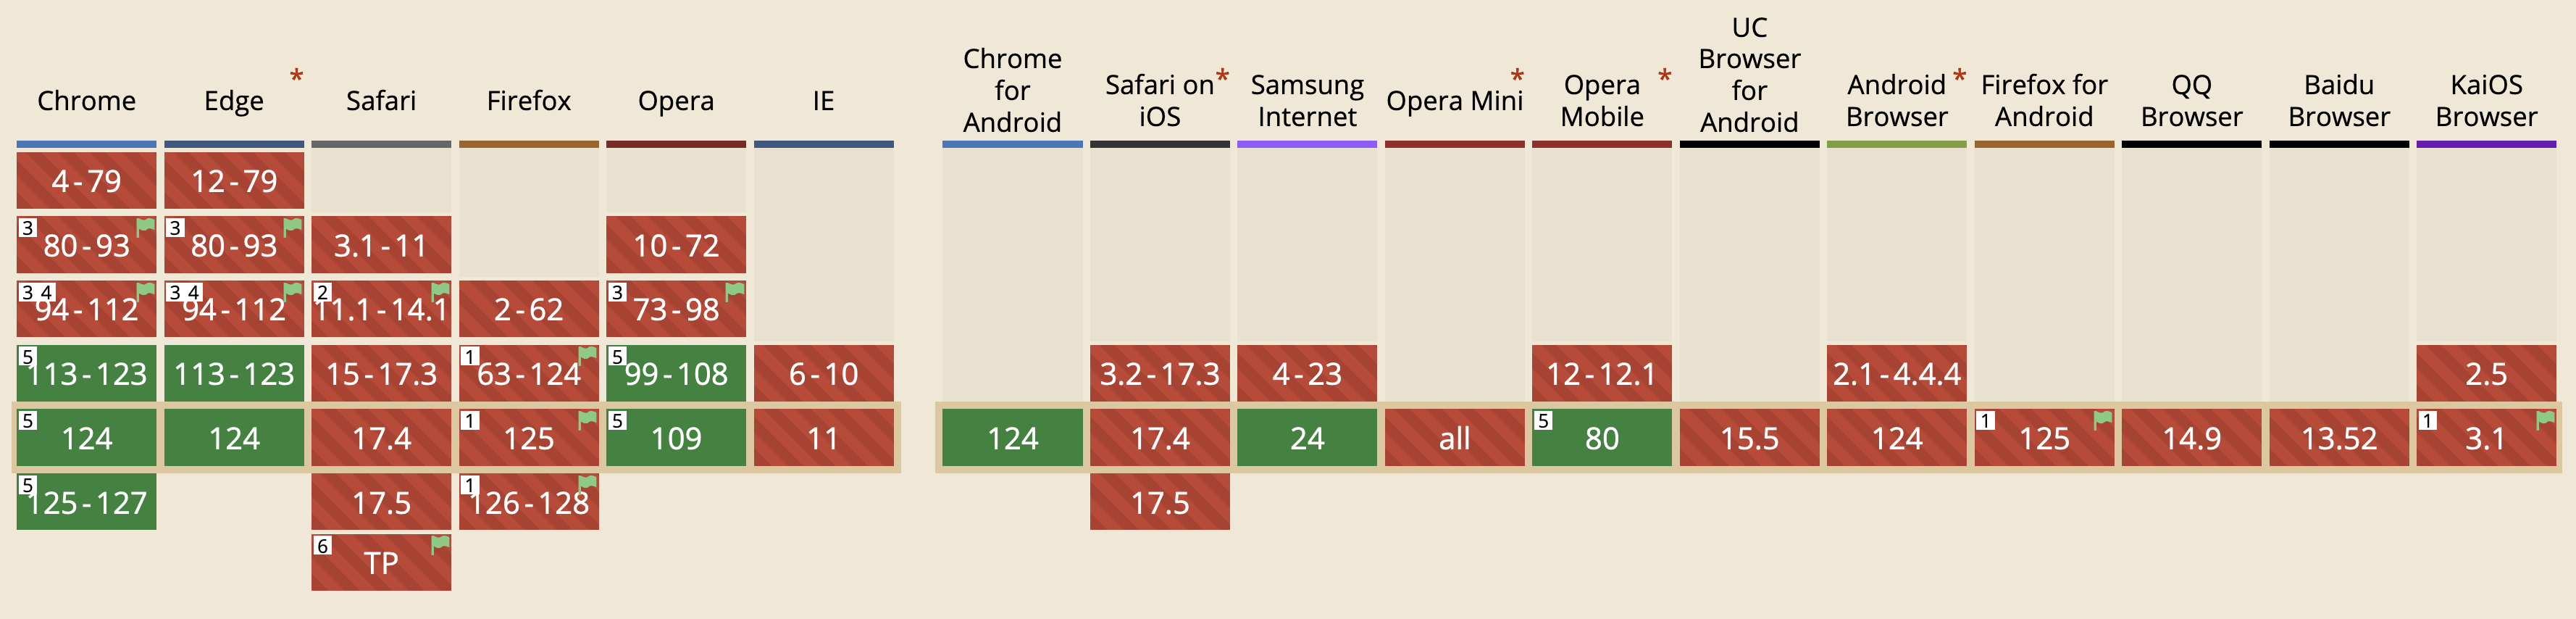
\includegraphics[width=\linewidth]{browsersupport.png}
    \caption{
        De \textit{Browser} ondersteuning voor \textit{WebGPU} te vinden op \href{https://caniuse.com/webgpu}{caniuse.com/webgpu}
        }{
            \textit{Browser} ondersteuning voor \textit{WebGPU}
        }
    \label{fig:Browser Support}
\end{figure}